\subsubsection{Scheduling multiple biopsies}
\label{subsubsec : pers_sched_algorithm}
Scheduling biopsies using personalized schedules is an iterative process. Only one biopsy is scheduled at once, using all the information available up to that point in time. The information is manifested via the predictive distribution $g(T^*_j)$. It is important to note that new biopsy times are only proposed when the patient visits the hospital for a PSA measurement or for biopsy, since $g(T^*_j)$ is updated only at these time points. If a biopsy is conducted at time $t$, then scheduling the next biopsy at time $u \geq \text{max}(t,s)$ for patient $j$ is the goal. Although the predictive distribution $g(T^*_j)$ is updated with the new information $T^*_j > t$, there are a couple of restrictions on time $u$, namely:

\begin{enumerate}
\item Two consecutive biopsies should have a gap of at least 1 year between them. i.e. $u \geq t + 1$. Given the medical side effects of biopsies, the 1 year gap is strongly advised for patients enrolled in PRIAS. However, the personalized scheduling methods do not take this rule into account.
\item Although it is required that $u \geq \text{max}(t,s)$, the personalized scheduling methods may propose to perform a biopsy at a time $u \epsilon (t, s]$. The reason is that, GR is not a terminating event, and so the patients continue to visit for PSA measurements. The support of the predictive distribution $g(T^*_j)$, however does not depend on last time of PSA measurement $s$, and remains $(t, \infty)$.
\end{enumerate}
 
Lastly, it is extremely likely that on consecutive visits to the hospital for PSA measurements, the personalized biopsy time is postponed or preponed. The choice of time of biopsy from consecutive visits is not clear. To resolve these issues, we propose to supplement the personalized scheduling methods with the following algorithm.


The variance however depends on both $t$ and $\mathcal{Y}_j(s)$. To elucidate the relationship between variance and observed information, we computed the variance at different time points for a couple of patients from the PRIAS study. The corresponding joint model fitted to the data set is discussed in Section \ref{subsec : jm_fit_prias}. The first patient in question is patient nr. 2340. He visited the hospital 34 times and was then right censored. 4 out those 34 visits were for biopsies. The variance of predictive distribution after each of those visits is shown in Figure \ref{fig : variance_pred_dist}. It is clear that the variance drops by a large margin each time a repeat biopsy is conducted. i.e. when more information about $T^*_j$ is available. The effect of $\mathcal{Y}_j(s)$ on variance can be seen in Figure \ref{fig : variance_pred_dist_3174} which corresponds to patient nr. 3174, who visited the hospital 9 times and was censored after his last biopsy. The observed PSA measurements for this patient are shown in Figure \ref{fig : observed_psa_3174}. It can be seen that the variance doesn't depend much on number of PSA measurements, but rather on the PSA values. For patient nr. 3174, variance drops quickly when PSA measurements increase sharply.  This becomes intuitive when we look at the model parameter estimates (Section \ref{subsec : param_estimates_jm_fit_prias}), where PSA velocity $m'_i(t)$ is a strong predictor of the hazard of GR.

\begin{figure}[!htb]
    \centering
    \captionsetup{justification=centering}
    \begin{subfigure}[b]{0.45\textwidth}
        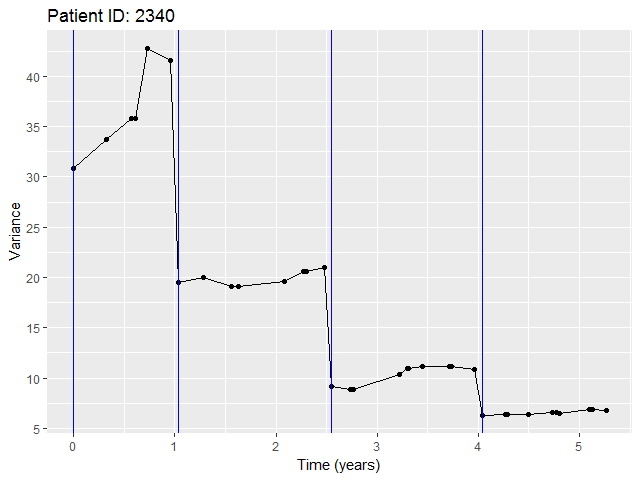
\includegraphics[width=\textwidth]{images/variance/variance_pred_dist_2340.png}
        \caption{Variance of the predictive distribution $g(T^*_j)$ over a period of 9 years for patient 2340. Blue vertical lines indicate biopsies.}
        \label{fig : variance_pred_dist_2340}
    \end{subfigure}   
    \begin{subfigure}[b]{0.45\textwidth}
        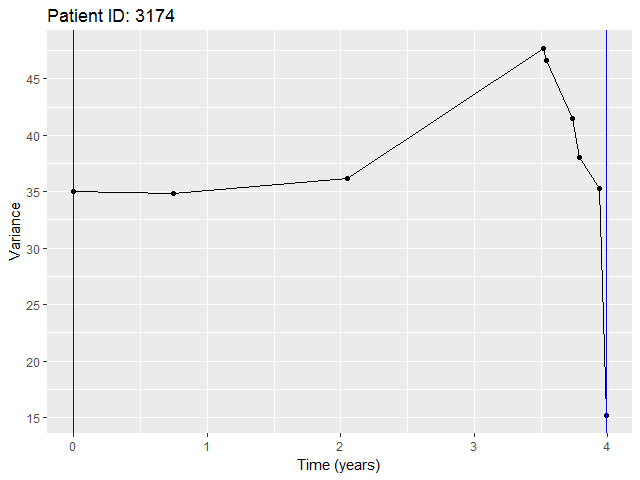
\includegraphics[width=\textwidth]{images/variance/variance_pred_dist_3174.png}
        \caption{Variance of the predictive distribution $g(T^*_j)$ over a period of 4 years for patient 3174. Blue vertical lines indicate biopsies.}
        \label{fig : variance_pred_dist_3174}
    \end{subfigure}
    \caption{Variance of the predictive distribution $g(T^*_j)$}\label{fig : variance_pred_dist}
\end{figure}

\begin{figure}[!htb]
    \centering
    \captionsetup{justification=centering}
    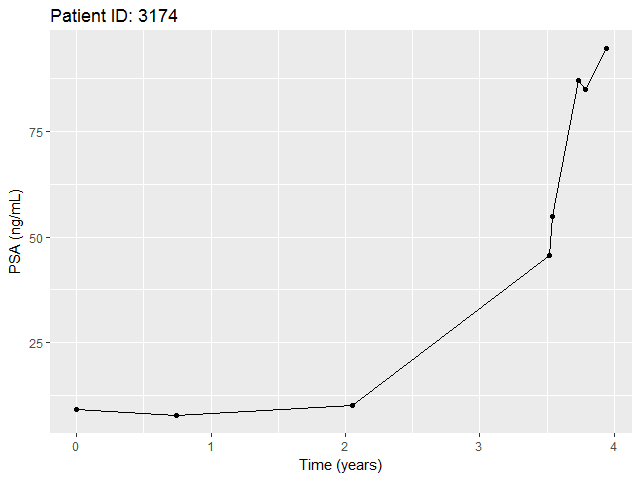
\includegraphics[width=0.5\textwidth]{images/observed_psa_3174.png}
    \caption{Observed evolution of PSA for patient 3174.}
    \label{fig : observed_psa_3174}
\end{figure}